% !TeX spellcheck = en_GB
% !TEX root = ../thesis.tex

\chapter{Details on the spin detection scheme} \label{app:spins_expt}

In this Appendix, give a few more practical details on the performance of the spin detection scheme presented in Chapter \ref{ch:spins}. 

\section{The effect of nonlinearities on normal modes}
\label{app:nonlin}

The transformation in Eq.~\eqref{eq:transform} can be applied to the nonlinear equation of motion, although this no longer decouples $x_S$ and $x_A$. Taking the difference $x_1 - x_2$ from Eqs.~\eqref{eq:x1} and~\eqref{eq:x2}, we obtain, after rearranging and leaving out the noise terms,
\begin{multline} \label{eq:fullnonlin}
\ddot{x}_A + \bigg[\gamma + \frac{\Gamma_1}{2} (x_S^2 + x_A^2) + \frac{\Gamma_2}{2} (3 \dot{x}_S^2 + \dot{x}_A^2)\bigg] \dot{x}_A \\ 
+ \bigg[\omega_0^2 + 2 \omega_0 \Delta \omega + \frac{\alpha}{2 m} x_A^2 + \frac{3 \alpha}{2 m} x_S^2 + \Gamma_1 x_S \dot{x}_S \bigg] x_A  \\ 
= \frac{M(t) \partial_x^2 B}{2 m} (x_S + x_A) + \frac{F(t)}{\sqrt{2} m}\,.
\end{multline}

Since $x_S \gg x_A$, we can drop all higher-order $x_A$ terms in Eq.~\eqref{eq:fullnonlin}. The readout mode thus behaves as a linear oscillator, but with an $x_S$-dependent damping and spring constant. Nonlinearity of the mode $x_S$ itself plays no role in the detection mechanism, we can thus continue to write its amplitude as $x_S = X_S \cos(\omega_S t)$. Eq.~\eqref{eq:fullnonlin} hence simplifies to the form used in Sec.~\ref{sec:nl}.

We note that in general, the pump mode $x_S$ is subject to thermal noise. Looking at the prefactor of $x_A$ in Eq.~\eqref{eq:fullnonlin}, we see this is converted to frequency noise of $x_A$ via the Duffing nonlinearity $\alpha$~\cite{Kenig_2012, Villanueva_2013, Yurke_1995}. Let us describe the noisy pump by $X_S = (X_{S0} + \delta X_S)  \cos(\omega_S t)$, where the $\delta X_S$ is the stochastic contribution of thermal noise. To leading order, this affects the frequency of $x_A$,
\begin{equation}
\omega_A^2 = \omega_0^2 + 2 \omega_0 \Delta \omega + \frac{3 \alpha}{m} X_{S0}  \, \delta X_S \cos^2(\omega_S t) \,.
\end{equation}
Taking $\expval{\delta X_S} = 0$ and $\expval{\delta X_S^2} = k_B T /  m \omega_S^2$ and dropping the oscillatory off-resonant terms, this introduces a variance of the frequency $\omega_A^2$,
\begin{equation}
\text{Var}(\omega_A^2) = \frac{3}{8} \left(\frac{3 \alpha}{m}\right)^2 \, X_{S0}^2 \, \expval{\delta X_S^2} \,.
\end{equation}
For the reference values in Appendix~\ref{app:vals} and $X_{S0} = 10$~nm, we obtain $\text{Var}(\omega_A^2) = 1.4\cross10^7$~s$^{-4}$. While this is far higher than the intrinsic frequency noise, it does not significantly diminish the resonant response of $x_A$ [cf. Eq.~\eqref{eq:varomega}].


\section{Spurious parametric terms in the nonlinear regime} \label{app:parametric}

Exciting the pump mode imparts multiple parametric drives on the readout mode, cf. Eqs.~\eqref{eq:omeganl} and~\eqref{eq:lambdas}. The effect of parametric driving is well-explored in the resonant case, where the spring constant is varied at twice the resonator's natural frequency~\cite{Cleland_2005}. The response amplitude in that case increases or decreases depending on the relative phase of the parametric and external drives, a phenomenon known as parametric squeezing~\cite{Lifshitz_2008}. 

In Eq.~\eqref{eq:omeganl} however, the spurious parametric terms oscillate at $2 \omega_S$ and are thus strongly detuned from $2\omega_A$. A straightforward perturbative treatment then shows that the drive induces spurious motion at frequencies $\abs{\omega_A \pm 2 \omega_S}$. The signal -- extracted from the Fourier component at $\omega_A$ -- is therefore unaffected. The result calculated earlier for the linear regime remains valid even in the presence of nonlinearities, with $Q$ replaced by $Q_{\rm nl}$. It is in principle possible for the drives to cause parametric instabilities, however, as our prospective system is far from the unstable regime, we do not pursue this issue further.

\section{Magnetic field simulations} \label{app:fields}
The magnetic field profile was estimated by modelling a hollow conical tip with a rounded top [cf. Fig.~\ref{fig:fields} (a)] with the magnetostatics package RADIA~\cite{Chubar_1998}. The tip was assumed to be magnetized to 1.83\;T parallel to the $x$-axis~\cite{Grob_2019}. A plot of the spatial profile of the second field gradient $\frac{\partial^2 B_x}{\partial x ^2}$ is shown in Fig.~\ref{fig:fields}(b). At 50\;nm above the tip center, we obtain $\frac{\partial ^2 B_x}{\partial x^2} = 2\cross10^{14}$ T\;m\textsuperscript{-2}.  

\begin{figure}
	\centering
	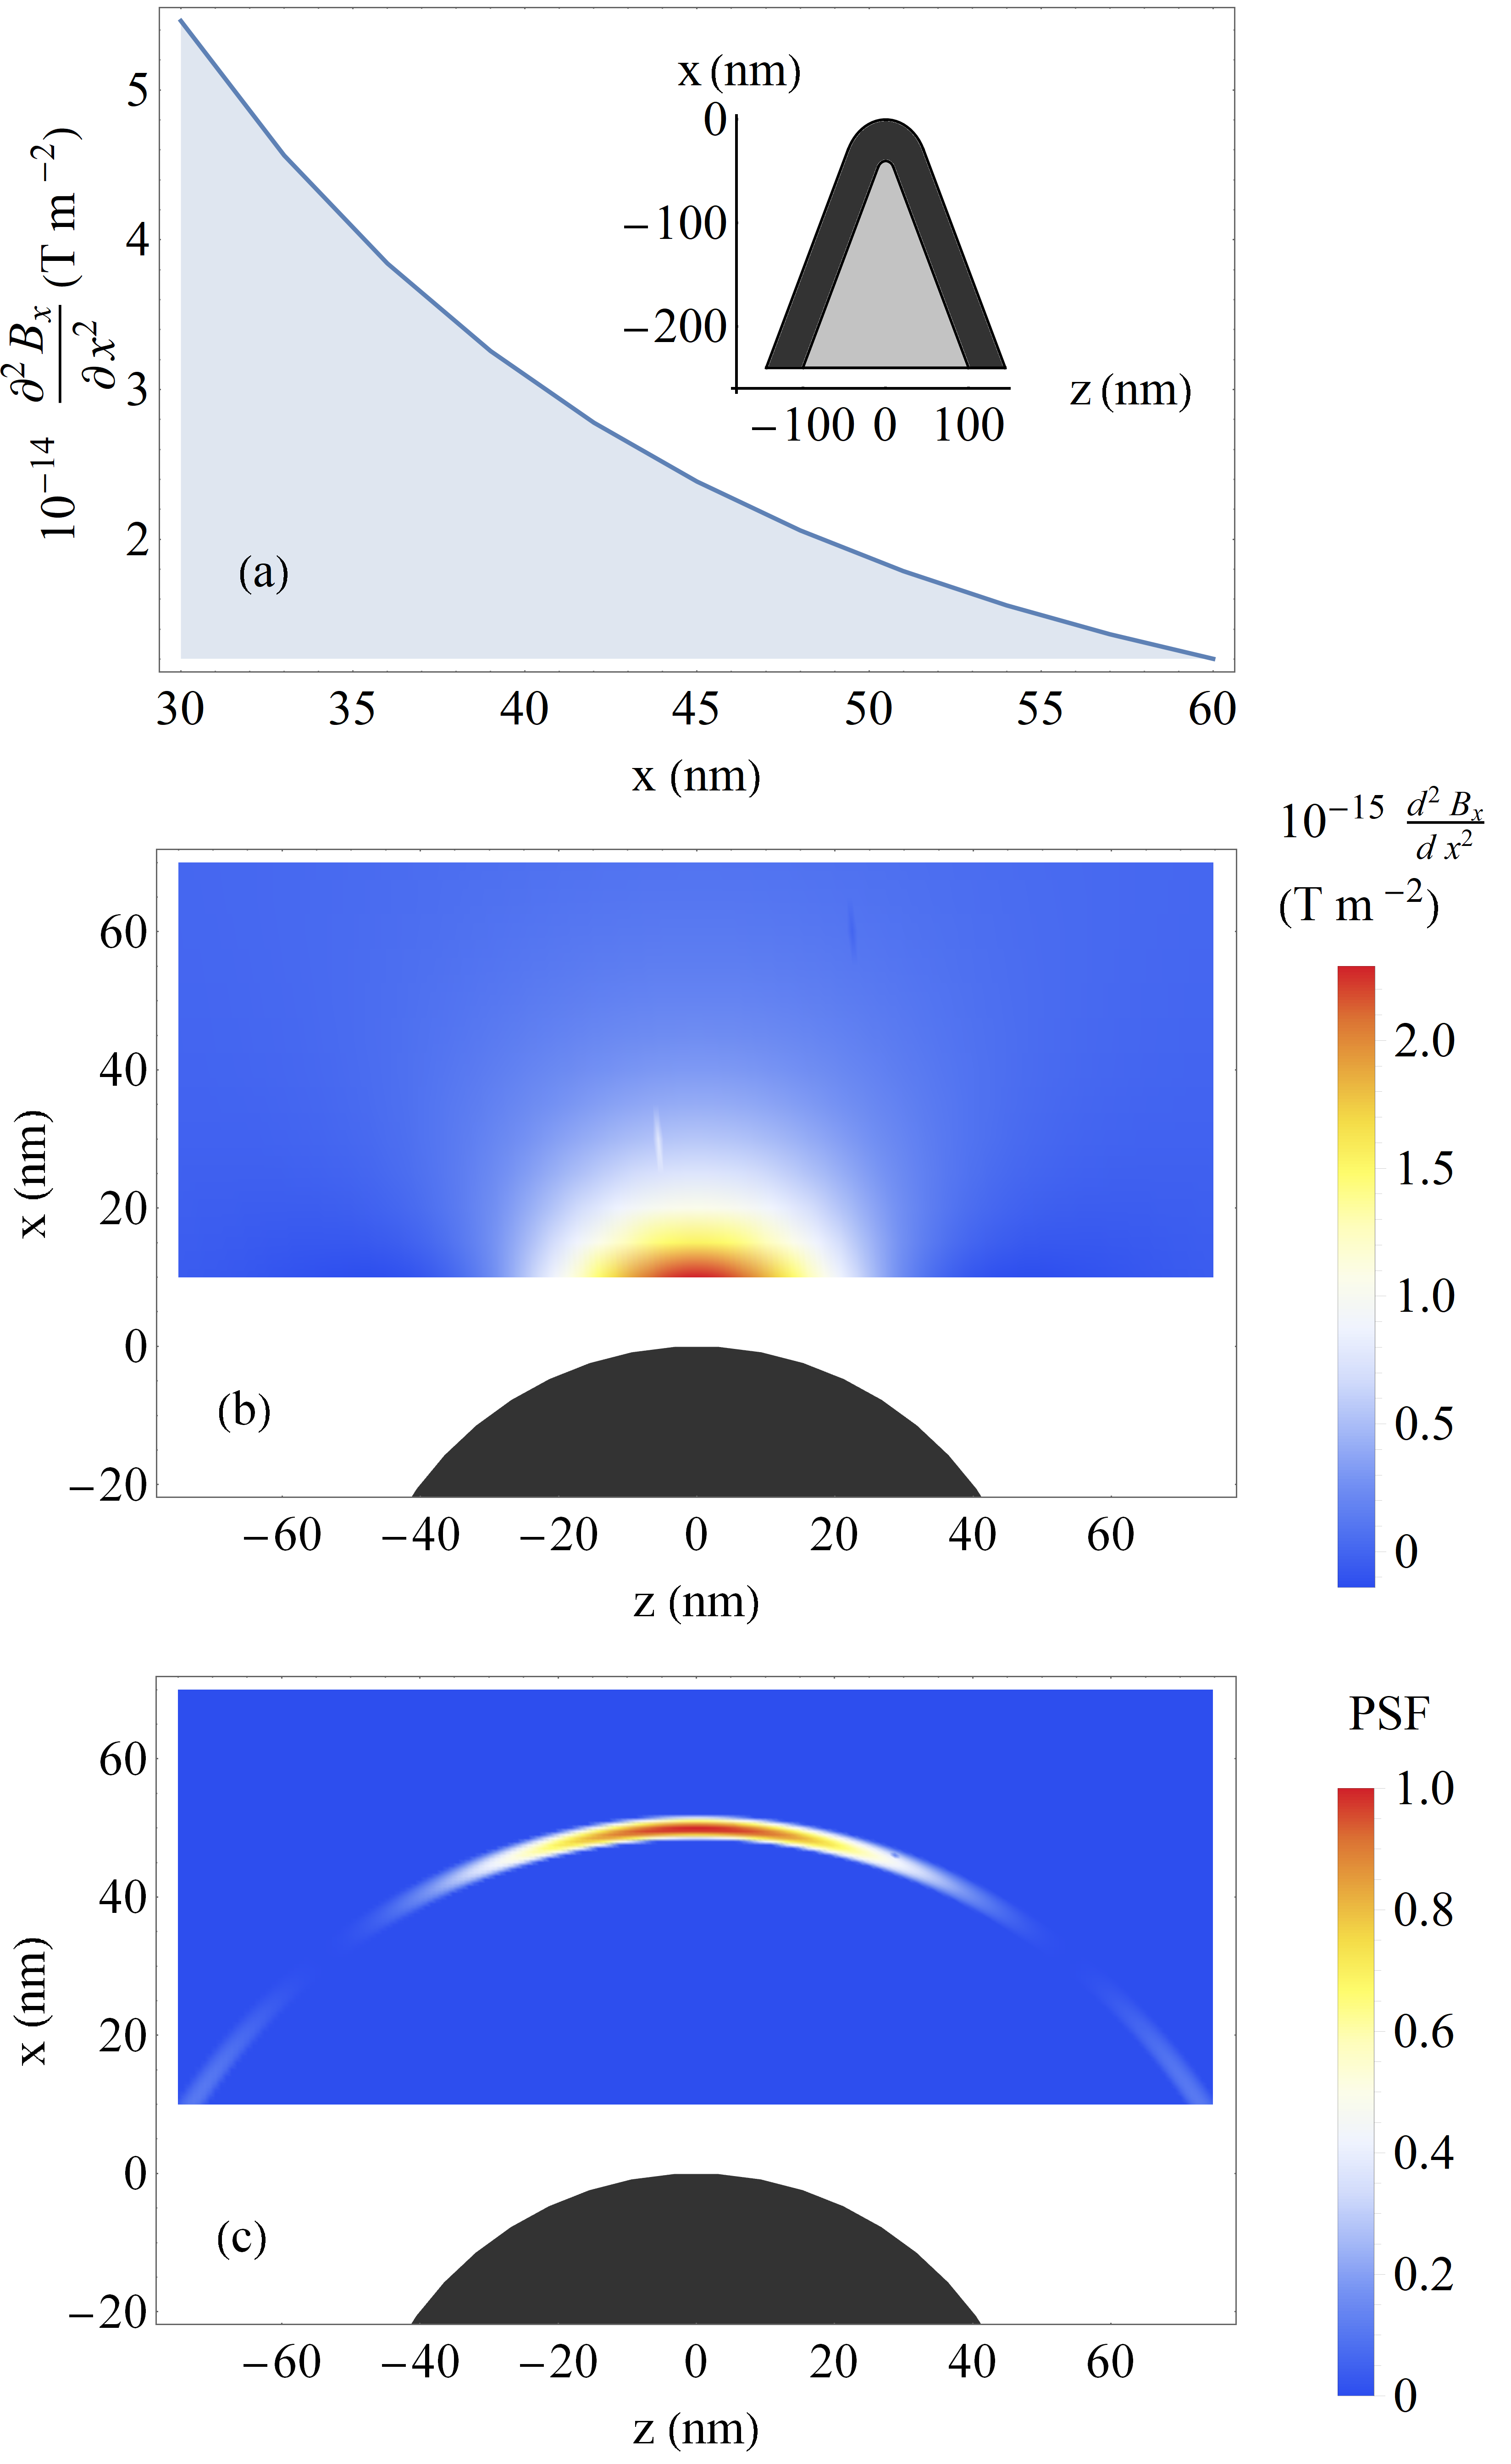
\includegraphics[width=0.78\columnwidth]{figures/spins/fig5.png}
	\caption{Magnetic field modelling results. (a) The second field gradient along the central axis of the magnetic tip; (inset) cross-section of the tip model, consisting of a non-magnetic conical base (light grey) and a layer of magnetic material (dark grey); (b) simulated second field gradient in the central plane of symmetry; (c) simulated PSF [cf. Eq.~\eqref{eq:PSF}], normalized to the value at 50\;nm above tip center. $\Delta \omega_{\rm rf} / \gamma_n = $ 10 mT was used.}
	\label{fig:fields}
\end{figure}

In an MRFM experiment, the spin-containing voxels constituting the sample cannot be scanned individually in real space. Instead, the frequency $\omega_{\rm rf}$ of the RF spin-flipping field is swept from $\omega_{\rm rf,0}-\Delta\omega_{\rm rf}$ to $\omega_{\rm rf,0}+\Delta\omega_{\rm rf}$. Spins whose Larmor frequency lies within these bounds are flipped, producing a signal proportional to the second field gradient, see Sec.~\ref{sec:spins_model}. The signal magnitude due to a spin at position $\vb{r}$ is hence a function of space, known as the point spread function (PSF). Here, we define the PSF as
\begin{equation} \label{eq:PSF}
\text{PSF}(\vb{r}) = \bigg[\frac{\partial^2 B_x (\vb{r})}{\partial x^2}\bigg]^2
\bigg[1-\bigg(\frac{\gamma_n |\vb{B}(\vb{r})| - \omega_{\rm rf,0}}{\Delta\omega_{\rm rf}}\bigg)^2\bigg]
\end{equation}
for $\gamma_n |\vb{B}(\vb{r}) - B_0| \leq \Delta \omega_{\rm rf}$ and 0 otherwise, with $\gamma_n$ being the nuclear spin gyromagnetic ratio. The bracketed term is an empirical expression describing flipping fidelity, whereby spins further off the central resonant condition produce less signal~\cite{Degen_2009}.

We plot the PSF in Fig.~\ref{fig:fields} (c), using for $\omega_{\rm rf,0}$ the Larmor frequency 50\;nm above the tip center. Note that in conventional MRFM, where the transducer is a cantilever moving along the $z$-axis, the relevant gradient would be $\frac{\partial B_x}{\partial z}$, which results in PSF maxima near the edges of the tip~\cite{Degen_2009}. With our proposed method based on $\frac{\partial B_x}{\partial x}$, these maxima persist but cannot be used due to the vertical motion of the membrane. We however find an additional active area on the central axis of the magnetic tip which makes for a feasible sample position. 

\section{Spin dynamics on the moving membrane} \label{app:spins}
A conceivable drawback of our spin detection scheme is the impact of the high pump mode amplitude, as well as the thermal motion of the membrane, on the spin ensemble. Since the ensemble moves rapidly through a region with a field gradient, its lifetime may be decreased by undergoing non-adiabatic dynamics. In particular, the effect of thermal noise has previously been found important in the context of cantilever-based MRFM~\cite{Berman_2003, Mozyrsky_2003}. 

We describe the flipping in the frame rotating with the Larmor frequency about the $x$-axis, where, under the effect of an applied RF field $B_{\rm rf}(t) \cos[\omega_{\rm rf} (t)]\: \hat{\vb{e}}_z$, the effective field reads
\begin{equation}
\vb{B}_{\rm rf}(t) = \mqty(\omega_{\rm rf}(t) / \gamma_n \\0 \\ B_{\rm rf}(t) )
\end{equation}
with the spin dynamics being governed by the Bloch equation,
\begin{equation} \label{eq:bloch}
\dot{\vb{M}}(t) = \gamma_n \vb{M}(t) \cross \vb{B}_{\rm rf}(t) .
\end{equation}
Starting with $\vb{B}_{\rm rf} (t)$ parallel to $x$-axis, a spin-flip is achieved by an adiabatic sweep across the Larmor frequency. For simplicity, we take a sinusoidal RF profile,
\begin{equation}
\vb{B}_{\rm rf}(t) = B_{\rm rf}\mqty(\cos{\Delta \omega t} \\ 0 \\ \sin{\Delta \omega t})
\end{equation}
with $B_{\rm rf} = $ 5\;mT~\cite{Grob_2019} and $\Delta\omega = \omega_A - \omega_S$ = $5\cross10^4$\;s\textsuperscript{-1}. Optimizing the pulse profiles will likely provide even more stable spin inversions~\cite{Grob_2019}.
\\

\textbf{Motion of the pump mode.} When the pump mode oscillates with amplitude $X_S$ [cf. Eqs.~\eqref{eq:transform}~and~\eqref{slowflow}], the sample position is $x_1(t) =  X_S \cos{\omega_S t} / \sqrt{2}$. Such a motion is equivalent to a spurious time-dependent field
\begin{equation}
\delta \vb{B}(t) = \frac{X_S}{\sqrt{2}} \frac{\partial B_x}{\partial x} \cos{\omega_S t}\: \hat{\vb{e}}_x \;.
\end{equation}
We solve Eq.~\eqref{eq:bloch} numerically with the field $\vb{B}_{\rm rf}(t) + \delta \vb{B}(t)$. From the field modelling in Appendix~\ref{app:fields}, we obtain $\frac{\partial B_x}{\partial x}=6\cross10^6$ T~m\textsuperscript{-1}.

Fig.~\ref{fig:flips} shows the flipping process under increasing values of $X_S$. We observe that the spurious field induces oscillatory features in the flipping process, but only causes significant distortion at very strong ($X_S \approx$ 100\;nm) pumping.

Finally, to test the flipping fidelity, we integrated Eq.~\ref{eq:bloch} over 250 flips using $X_S=$ 10\;nm. Starting with a unit vector $\vb{M}(0)=\hat{\vb{e}}_x$, the magnetization $M_x$ at the end of each flip never dropped below 0.996. We thus conclude the flipping mechanism remains robust under strong driving of the pump mode.
\\

\begin{figure}
	\centering
	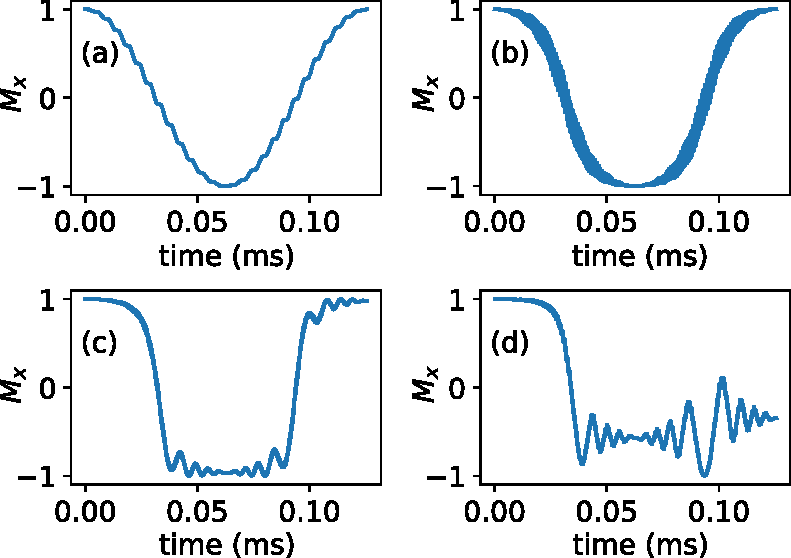
\includegraphics[width=0.65\columnwidth]{figures/spins/fig6_revised.pdf}
	\caption{Magnetization component along the $x$-axis in the flipping process under increasing values of the pump amplitude. (a) $X_S$ = 0, (b) $X_S$ = 10\;nm, (c) $X_S$ = 50\;nm, (d) $X_S$ = 100\;nm.}
	\label{fig:flips}
\end{figure}

\textbf{Thermal noise in the membrane.} We measured the thermal displacement on one of the defect mode sites of a Si\textsubscript{3}N\textsubscript{4} membrane. At room temperature, a root-mean-square displacement of 150~pm was observed, most of which was due to the many delocalized modes of the membrane. Since cantilever-based MRFM displays high flipping fidelities at comparable displacement noise levels, and since our envisioned operational temperature (0.2 K) will further reduce thermal fluctuations, we do not expect this to be an issue with regards to spin-flipping.
\\

\section{Reference values} \label{app:vals}
All resonator parameters used in Sec.~\ref{sec:spins_disc} are shown in Table~\ref{table:spins_params}. The values are taken from recent experimental data~\cite{Catalini_2020}. Note that a different, non-unitary normal mode transformation is typically used in experimental literature,
\begin{equation}
\mqty(x_S \\ x_A) = \mqty(1 && 1 \\ 1 && -1) \mqty(x_1 \\ x_2)\,. 
\end{equation}
Relative to our notation, this scales the cubic nonlinearities $\alpha, \Gamma_{\rm nl}$ by a factor of $\frac{1}{2}$ and the mass $m$ by a factor of 2. This transformation is convenient for experimental use, but requires additional renormalization when dealing with external forces.

The magnetic field gradients were estimated by modelling a conical magnetic tip made of saturated NdFeB  magnet (such as is used in MFM) with the magnetostatics package RADIA~\cite{Chubar_1998}. The sample is assumed to be positioned directly above the center of the magnetic tip, where there is a relatively large area of constant $\partial^2_x B$. 

%\begin{widetext}
%	\label{table:spins_params}
	\begin{center}
		\begin{table} [h!]
			\caption{Reference resonator parameters and magnetic field characteristics.}
			\label{table:spins_params}
			\def\arraystretch{1.3}
			\begin{tabular}{|  m{2.8cm} |  m{1.9cm} | m{4.8cm} |}
				\hline
				$m$ (ng) & 1 & resonator mass  \\ 
				\hline
				$\omega_0$ (s$^{-1}$)& $8.2 \cross 10^6$ & resonator natural frequency\\ 
				\hline
				$Q$ & $10^8$ & quality factor  \\
				\hline
				$\alpha$ (kg m$^{-2}$ s$^{-2}$) & $1 \cross 10^{12}$ & coefficient of Duffing nonlinearity \\
				\hline
				$\omega_A - \omega_S$ (s$^{-1}$) & $5 \cross 10^4$ & normal mode frequency splitting\\
				\hline
				Var($x_1$) (m\textsuperscript{2}) & $2.2 \cross 10^{-20}$ &  thermal displacement variance at room temperature \\
				
				\hline
				$\partial_x B$ (T m$^{-1}$) & $6 \cross 10^{6}$ & magnetic field gradient $\frac{\partial B_x}{\partial x}$\\
				\hline
				$\partial_x^2 B$ (T m$^{-2}$) & $2 \cross 10^{14}$ & second magnetic field gradient $\frac{\partial^2 B_x}{\partial x^2}$ \\
				\hline
				$\eta$ & $0.5$ & detection efficiency \\
				\hline
				$S_{\rm det}$ (m$^2$~s) & $10^{-31}$ & detector noise PSD \\
				\hline
				Var($\omega_A^2$) (s$^{-4}$) & 10$^{-1}$ & frequency variance due to intrinsic frequency noise\\
				\hline
				$S_\chi(\omega_A -\omega_S )$ (s$^{-1}$) & $\leq 10^{-36} $ & relative intrinsic frequency noise PSD at resonance \\
				\hline
			\end{tabular}
		\end{table}
	\end{center}
%\end{widetext}
